
%% bare_conf.tex
%% V1.4
%% 2012/12/27
%% by Michael Shell
%% See:
%% http://www.michaelshell.org/
%% for current contact information.
%%
%% This is a skeleton file demonstrating the use of IEEEtran.cls
%% (requires IEEEtran.cls version 1.8 or later) with an IEEE conference paper.
%%
%% Support sites:
%% http://www.michaelshell.org/tex/ieeetran/
%% http://www.ctan.org/tex-archive/macros/latex/contrib/IEEEtran/
%% and
%% http://www.ieee.org/

%%*************************************************************************
%% Legal Notice:
%% This code is offered as-is without any warranty either expressed or
%% implied; without even the implied warranty of MERCHANTABILITY or
%% FITNESS FOR A PARTICULAR PURPOSE! 
%% User assumes all risk.
%% In no event shall IEEE or any contributor to this code be liable for
%% any damages or losses, including, but not limited to, incidental,
%% consequential, or any other damages, resulting from the use or misuse
%% of any information contained here.
%%
%% All comments are the opinions of their respective authors and are not
%% necessarily endorsed by the IEEE.
%%
%% This work is distributed under the LaTeX Project Public License (LPPL)
%% ( http://www.latex-project.org/ ) version 1.3, and may be freely used,
%% distributed and modified. A copy of the LPPL, version 1.3, is included
%% in the base LaTeX documentation of all distributions of LaTeX released
%% 2003/12/01 or later.
%% Retain all contribution notices and credits.
%% ** Modified files should be clearly indicated as such, including  **
%% ** renaming them and changing author support contact information. **
%%
%% File list of work: IEEEtran.cls, IEEEtran_HOWTO.pdf, bare_adv.tex,
%%                    bare_conf.tex, bare_jrnl.tex, bare_jrnl_compsoc.tex,
%%                    bare_jrnl_transmag.tex
%%*************************************************************************

% *** Authors should verify (and, if needed, correct) their LaTeX system  ***
% *** with the testflow diagnostic prior to trusting their LaTeX platform ***
% *** with production work. IEEE's font choices can trigger bugs that do  ***
% *** not appear when using other class files.                            ***
% The testflow support page is at:
% http://www.michaelshell.org/tex/testflow/



% Note that the a4paper option is mainly intended so that authors in
% countries using A4 can easily print to A4 and see how their papers will
% look in print - the typesetting of the document will not typically be
% affected with changes in paper size (but the bottom and side margins will).
% Use the testflow package mentioned above to verify correct handling of
% both paper sizes by the user's LaTeX system.
%
% Also note that the "draftcls" or "draftclsnofoot", not "draft", option
% should be used if it is desired that the figures are to be displayed in
% draft mode.
%
\documentclass[11pt,conference]{IEEEtran}
% Add the compsoc option for Computer Society conferences.
%
% If IEEEtran.cls has not been installed into the LaTeX system files,
% manually specify the path to it like:
% \documentclass[conference]{../sty/IEEEtran}

\usepackage{amsmath}
\usepackage{amssymb}

\usepackage{textcomp}

\usepackage[ruled, vlined, boxed]{algorithm2e}
\usepackage{booktabs}

\usepackage{algorithmic}

\usepackage{amsfonts}

%%%%%

%\usepackage{marvosym}
\usepackage{bm}
\usepackage{amsmath}   % From the American Mathematical Society

%\usepackage{algorithm}

\usepackage{amsfonts}
\usepackage{latexsym}
\usepackage{amssymb}
\usepackage{amsthm}
\usepackage{color}
\usepackage[colorlinks,urlcolor=magenta]{hyperref}
%\usepackage[linesnumbered,boxed]{algorithm2e}



% Some very useful LaTeX packages include:
% (uncomment the ones you want to load)

% *** MISC UTILITY PACKAGES ***
%
%\usepackage{ifpdf}
% Heiko Oberdiek's ifpdf.sty is very useful if you need conditional
% compilation based on whether the output is pdf or dvi.
% usage:
% \ifpdf
%   % pdf code
% \else
%   % dvi code
% \fi
% The latest version of ifpdf.sty can be obtained from:
% http://www.ctan.org/tex-archive/macros/latex/contrib/oberdiek/
% Also, note that IEEEtran.cls V1.7 and later provides a builtin
% \ifCLASSINFOpdf conditional that works the same way.
% When switching from latex to pdflatex and vice-versa, the compiler may
% have to be run twice to clear warning/error messages.






% *** CITATION PACKAGES ***
%
\usepackage{cite}
% cite.sty was written by Donald Arseneau
% V1.6 and later of IEEEtran pre-defines the format of the cite.sty package
% \cite{} output to follow that of IEEE. Loading the cite package will
% result in citation numbers being automatically sorted and properly
% "compressed/ranged". e.g., [1], [9], [2], [7], [5], [6] without using
% cite.sty will become [1], [2], [5]--[7], [9] using cite.sty. cite.sty's
% \cite will automatically add leading space, if needed. Use cite.sty's
% noadjust option (cite.sty V3.8 and later) if you want to turn this off
% such as if a citation ever needs to be enclosed in parenthesis.
% cite.sty is already installed on most LaTeX systems. Be sure and use
% version 4.0 (2003-05-27) and later if using hyperref.sty. cite.sty does
% not currently provide for hyperlinked citations.
% The latest version can be obtained at:
% http://www.ctan.org/tex-archive/macros/latex/contrib/cite/
% The documentation is contained in the cite.sty file itself.






% *** GRAPHICS RELATED PACKAGES ***
%
\ifCLASSINFOpdf
 \usepackage[pdftex]{graphicx}
  % declare the path(s) where your graphic files are
  % \graphicspath{{../pdf/}{../jpeg/}}
  % and their extensions so you won't have to specify these with
  % every instance of \includegraphics
 %\DeclareGraphicsExtensions{.pdf,.jpeg,.png}
\else
  % or other class option (dvipsone, dvipdf, if not using dvips). graphicx
  % will default to the driver specified in the system graphics.cfg if no
  % driver is specified.
 \usepackage[dvips]{graphicx}
  % declare the path(s) where your graphic files are
 \graphicspath{{../}}
  % and their extensions so you won't have to specify these with
  % every instance of \includegraphics
 \DeclareGraphicsExtensions{.eps}
\fi
% graphicx was written by David Carlisle and Sebastian Rahtz. It is
% required if you want graphics, photos, etc. graphicx.sty is already
% installed on most LaTeX systems. The latest version and documentation
% can be obtained at: 
% http://www.ctan.org/tex-archive/macros/latex/required/graphics/
% Another good source of documentation is "Using Imported Graphics in
% LaTeX2e" by Keith Reckdahl which can be found at:
% http://www.ctan.org/tex-archive/info/epslatex/
%
% latex, and pdflatex in dvi mode, support graphics in encapsulated
% postscript (.eps) format. pdflatex in pdf mode supports graphics
% in .pdf, .jpeg, .png and .mps (metapost) formats. Users should ensure
% that all non-photo figures use a vector format (.eps, .pdf, .mps) and
% not a bitmapped formats (.jpeg, .png). IEEE frowns on bitmapped formats
% which can result in "jaggedy"/blurry rendering of lines and letters as
% well as large increases in file sizes.
%
% You can find documentation about the pdfTeX application at:
% http://www.tug.org/applications/pdftex





% *** MATH PACKAGES ***
%
%\usepackage[cmex10]{amsmath}
% A popular package from the American Mathematical Society that provides
% many useful and powerful commands for dealing with mathematics. If using
% it, be sure to load this package with the cmex10 option to ensure that
% only type 1 fonts will utilized at all point sizes. Without this option,
% it is possible that some math symbols, particularly those within
% footnotes, will be rendered in bitmap form which will result in a
% document that can not be IEEE Xplore compliant!
%
% Also, note that the amsmath package sets \interdisplaylinepenalty to 10000
% thus preventing page breaks from occurring within multiline equations. Use:
%\interdisplaylinepenalty=2500
% after loading amsmath to restore such page breaks as IEEEtran.cls normally
% does. amsmath.sty is already installed on most LaTeX systems. The latest
% version and documentation can be obtained at:
% http://www.ctan.org/tex-archive/macros/latex/required/amslatex/math/





% *** SPECIALIZED LIST PACKAGES ***
%
\usepackage{algorithmic}
% algorithmic.sty was written by Peter Williams and Rogerio Brito.
% This package provides an algorithmic environment fo describing algorithms.
% You can use the algorithmic environment in-text or within a figure
% environment to provide for a floating algorithm. Do NOT use the algorithm
% floating environment provided by algorithm.sty (by the same authors) or
% algorithm2e.sty (by Christophe Fiorio) as IEEE does not use dedicated
% algorithm float types and packages that provide these will not provide
% correct IEEE style captions. The latest version and documentation of
% algorithmic.sty can be obtained at:
% http://www.ctan.org/tex-archive/macros/latex/contrib/algorithms/
% There is also a support site at:
% http://algorithms.berlios.de/index.html
% Also of interest may be the (relatively newer and more customizable)
% algorithmicx.sty package by Szasz Janos:
% http://www.ctan.org/tex-archive/macros/latex/contrib/algorithmicx/




% *** ALIGNMENT PACKAGES ***
%
%\usepackage{array}
% Frank Mittelbach's and David Carlisle's array.sty patches and improves
% the standard LaTeX2e array and tabular environments to provide better
% appearance and additional user controls. As the default LaTeX2e table
% generation code is lacking to the point of almost being broken with
% respect to the quality of the end results, all users are strongly
% advised to use an enhanced (at the very least that provided by array.sty)
% set of table tools. array.sty is already installed on most systems. The
% latest version and documentation can be obtained at:
% http://www.ctan.org/tex-archive/macros/latex/required/tools/


% IEEEtran contains the IEEEeqnarray family of commands that can be used to
% generate multiline equations as well as matrices, tables, etc., of high
% quality.




% *** SUBFIGURE PACKAGES ***
%\ifCLASSOPTIONcompsoc
%  \usepackage[caption=false,font=normalsize,labelfont=sf,textfont=sf]{subfig}
%\else
%  \usepackage[caption=false,font=footnotesize]{subfig}
%\fi
% subfig.sty, written by Steven Douglas Cochran, is the modern replacement
% for subfigure.sty, the latter of which is no longer maintained and is
% incompatible with some LaTeX packages including fixltx2e. However,
% subfig.sty requires and automatically loads Axel Sommerfeldt's caption.sty
% which will override IEEEtran.cls' handling of captions and this will result
% in non-IEEE style figure/table captions. To prevent this problem, be sure
% and invoke subfig.sty's "caption=false" package option (available since
% subfig.sty version 1.3, 2005/06/28) as this is will preserve IEEEtran.cls
% handling of captions.
% Note that the Computer Society format requires a larger sans serif font
% than the serif footnote size font used in traditional IEEE formatting
% and thus the need to invoke different subfig.sty package options depending
% on whether compsoc mode has been enabled.
%
% The latest version and documentation of subfig.sty can be obtained at:
% http://www.ctan.org/tex-archive/macros/latex/contrib/subfig/


% *** FLOAT PACKAGES ***
%
\usepackage{float}
%\usepackage{fixltx2e}
% fixltx2e, the successor to the earlier fix2col.sty, was written by
% Frank Mittelbach and David Carlisle. This package corrects a few problems
% in the LaTeX2e kernel, the most notable of which is that in current
% LaTeX2e releases, the ordering of single and double column floats is not
% guaranteed to be preserved. Thus, an unpatched LaTeX2e can allow a
% single column figure to be placed prior to an earlier double column
% figure. The latest version and documentation can be found at:
% http://www.ctan.org/tex-archive/macros/latex/base/


%\usepackage{stfloats}
% stfloats.sty was written by Sigitas Tolusis. This package gives LaTeX2e
% the ability to do double column floats at the bottom of the page as well
% as the top. (e.g., "\begin{figure*}[!b]" is not normally possible in
% LaTeX2e). It also provides a command:
%\fnbelowfloat
% to enable the placement of footnotes below bottom floats (the standard
% LaTeX2e kernel puts them above bottom floats). This is an invasive package
% which rewrites many portions of the LaTeX2e float routines. It may not work
% with other packages that modify the LaTeX2e float routines. The latest
% version and documentation can be obtained at:
% http://www.ctan.org/tex-archive/macros/latex/contrib/sttools/
% Do not use the stfloats baselinefloat ability as IEEE does not allow
% \baselineskip to stretch. Authors submitting work to the IEEE should note
% that IEEE rarely uses double column equations and that authors should try
% to avoid such use. Do not be tempted to use the cuted.sty or midfloat.sty
% packages (also by Sigitas Tolusis) as IEEE does not format its papers in
% such ways.
% Do not attempt to use stfloats with fixltx2e as they are incompatible.
% Instead, use Morten Hogholm'a dblfloatfix which combines the features
% of both fixltx2e and stfloats:
%
%\usepackage{dblfloatfix}
% The latest version can be found at:
% http://www.ctan.org/tex-archive/macros/latex/contrib/dblfloatfix/


% *** INSERT CODE PACKAGES***
\usepackage{listings}
\usepackage{color}

\definecolor{dkgreen}{rgb}{0,0.6,0}
\definecolor{gray}{rgb}{0.5,0.5,0.5}
\definecolor{mauve}{rgb}{0.58,0,0.82}

\lstset{frame=tb,
  language=Java,
  aboveskip=3mm,
  belowskip=3mm,
  showstringspaces=false,
  columns=flexible,
  basicstyle={\small\ttfamily},
  numbers=none,
  numberstyle=\tiny\color{gray},
  keywordstyle=\color{blue},
  commentstyle=\color{dkgreen},
  stringstyle=\color{mauve},
  breaklines=true,
  breakatwhitespace=true,
  tabsize=3
}

% *** PDF, URL AND HYPERLINK PACKAGES ***
%
%\usepackage{url}
% url.sty was written by Donald Arseneau. It provides better support for
% handling and breaking URLs. url.sty is already installed on most LaTeX
% systems. The latest version and documentation can be obtained at:
% http://www.ctan.org/tex-archive/macros/latex/contrib/url/
% Basically, \url{my_url_here}.




% *** Do not adjust lengths that control margins, column widths, etc. ***
% *** Do not use packages that alter fonts (such as pslatex).         ***
% There should be no need to do such things with IEEEtran.cls V1.6 and later.
% (Unless specifically asked to do so by the journal or conference you plan
% to submit to, of course. )


% correct bad hyphenation here
\hyphenation{op-tical net-works semi-conduc-tor}


\begin{document}
%
% paper title
% can use linebreaks \\ within to get better formatting as desired
% Do not put math or special symbols in the title.
\title{San Francisco Crime Classification and Prediction}

% author names and affiliations
% use a multiple column layout for up to three different
% affiliations
\author{\IEEEauthorblockN{Kai Wang}
\IEEEauthorblockA{Department of Computer Science, UCLA\\
{kwang42@cs.ucla.edu}}}

% conference papers do not typically use \thanks and this command
% is locked out in conference mode. If really needed, such as for
% the acknowledgment of grants, issue a \IEEEoverridecommandlockouts
% after \documentclass

% for over three affiliations, or if they all won't fit within the width
% of the page, use this alternative format:
% 
%\author{\IEEEauthorblockN{Michael Shell\IEEEauthorrefmark{1},
%Homer Simpson\IEEEauthorrefmark{2},
%James Kirk\IEEEauthorrefmark{3}, 
%Montgomery Scott\IEEEauthorrefmark{3} and
%Eldon Tyrell\IEEEauthorrefmark{4}}
%\IEEEauthorblockA{\IEEEauthorrefmark{1}School of Electrical and Computer Engineering\\
%Georgia Institute of Technology,
%Atlanta, Georgia 30332--0250\\ Email: see http://www.michaelshell.org/contact.html}
%\IEEEauthorblockA{\IEEEauthorrefmark{2}Twentieth Century Fox, Springfield, USA\\
%Email: homer@thesimpsons.com}
%\IEEEauthorblockA{\IEEEauthorrefmark{3}Starfleet Academy, San Francisco, California 96678-2391\\
%Telephone: (800) 555--1212, Fax: (888) 555--1212}
%\IEEEauthorblockA{\IEEEauthorrefmark{4}Tyrell Inc., 123 Replicant Street, Los Angeles, California 90210--4321}}




% use for special paper notices
%\IEEEspecialpapernotice{(Invited Paper)}


% make the title area
\maketitle

% As a general rule, do not put math, special symbols or citations
% in the abstract
\begin{abstract}
In this paper, we apply machine learning and time series analysis to the problem of classifying and forecasting crime incidents in San Francisco. Our dataset originates from a Kaggle competition \cite{1}. Based on existing researches on these problems, we employ Logistic Regression and VAR(p) models respectively. The classification problem result demonstrates high challenge as our results across all the 39 crime categories achieved the accuracy of 32.67\%. For the time series analysis, we revealed correlations of occurrences of difference crime categories. And the VAR(p) model can forecast the trend of number of certain crimes. We also involved demographic data for classification problem, which contributed to a slight improvement to accuracy. With richer and more up-to-date data, our results might be further improved.
\end{abstract}

% no keywords
{\bf Keywords: Crime Prediction; Feature Engineering; Classification; Time Series Analysis}


% For peer review papers, you can put extra information on the cover
% page as needed:
% \ifCLASSOPTIONpeerreview
% \begin{center} \bfseries EDICS Category: 3-BBND \end{center}
% \fi
%
% For peerreview papers, this IEEEtran command inserts a page break and
% creates the second title. It will be ignored for other modes.
\IEEEpeerreviewmaketitle


\section{Introduction}
Crime activities have always been threat to public safety, and researches on criminals have long been limited within the realm social science. With the huge volume of existing crime datasets and the advent of robust machine learning and statistical technologies, we seek to predictively analyze crime incidents. Our vision is to help police, public policy makers as well as individuals understand crime patterns and take more effective measures to prevent crimes.

In our project, we combined spatio-temporal and demographic data to predict which category of crime has the largest possibility to occur, given a timestamp, location and demographics of the surrounding area. The inputs to our classification algorithm include time (hour, day, year), location(street, latitude, longitude and police district) and demographic data(population density, median house value, poverty rate and median per capita income). The output is the type of crime that  is most likely to have occurred. We performed complicated feature engineering to enrich predictors. We also tried various classification algorithms, among which Logistic Regression achieved highest accuracy.

For time series analysis, we  applied vector autogression model to capture the interdependencies among multiple categories of crime time series. We tested for the optimal lag $p$ for VAR(p) model. The input to VAR(p) is spatio-temporal data; the output is the time series model. For some crime categories, this model can reveal the trends of its occurrence.

\section{Datasets}
Our primary dataset is a training set obtained from Kaggle, which includes 878,049 crimes in San francisco that occurred from 2003 to 2015. Every crime record was marked a category, and there are in total 39 categories. The other dataset is the demographic data of different neighborhoods in San Francisco, including population, income, race constitution, education level etc. The demographic data is provided by US Census conducted in 2010. We also searched Wikipedia for population density. 
\subsection{Features}
Each record in our dataset correspond to a particular crime incident, which includes following fields:
\begin{itemize}
  \item Date and timestamp of the crime
  \item Category of the crime. Which is the label to be predicted in test data set.
  \item Detailed description of the crime (only provided in train data)
  \item Day of the week of the incident
  \item Name of the Police Department District the took charge of the crime.
  \item Resolution, which means how the crime was resolved(booked, arrested or resolved, etc)
  \item Approximate street address of the crime
  \item Longitude
  \item Latitude
\end{itemize}
Among these fields, resolution is discarded as it only exist in train data.
\subsection{Preprocessing}
While \url{http://datasf.org} also includes similar data, our dataset from Kaggle is more selected as there is no empty cell in any fields. However, some fields contain unreasonable values due to probably wrong registration. Some numeric fields need to be scaled while some fields are not yet numeric. To transform the original data to suitable input of classification algorithms, we performed feature engineering described below.
\subsubsection{Outlier removal}
The following pictures in Fig.1 are scatter plots of scaled longitude(X) and latitude(Y). There are in total 67 outlier points, all of their latitudes are beyond the border of San Francisco. After removal of these outliers, the scatter plot fits the territory of San Francisco.
\begin{figure}[H]
\begin{center}
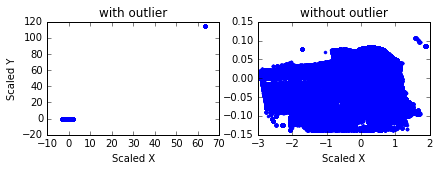
\includegraphics [width=0.48\textwidth]{pics/outliers.png}
\caption{Scatter plot of crime locations before and after outlier removal}
\end{center}
\end{figure}

\subsubsection{Demographic data}
Our demographic data is based on US Census from 2006 to 2010. It includes demographic data in each neighborhood of San Francisco, covering race, education, income and housing characteristics. The heatmap in Fig 2 displayed the correlation among the frequency of some typical crime categories and demographic statistics. For example, poverty rate is positively correlated to most crime categories, especially embezzlement; while high population density tend to relate to drug use and disorderly conduct.

One challenge of employing demographic data is correctly matching it the the crime location as the crime dataset does not include neighborhood. Our solution was to download the map data of San Francisco, where each neighborhood is represented as a polygon. Following pseudo-code shows how we located each neighborhood.
\begin{lstlisting}
bool getNeighborhood(Lang, Lat, Polygon){ 
	//For acceleration
	if (Lang, Lat) in Polygon-Bounding-Box{
		if (Lang, Lat) in Polygon{
			return True
		}
	}
	return False
}
\end{lstlisting}

\begin{figure}[H]
\begin{center}
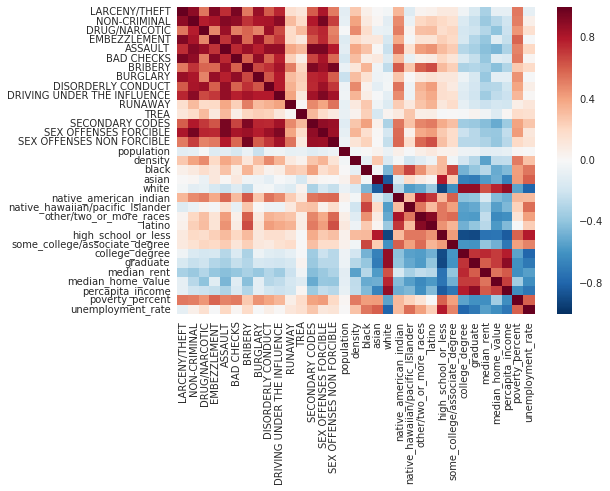
\includegraphics [width=0.48\textwidth]{pics/nh_category_corr.png}
\caption{heat map of correlation among crime amount and demographic data}
\end{center}
\end{figure}

\subsubsection{Feature enrichment}
For timestamps in dataset, we parsed the month\/date-of-year, hour-of-day from them. We also added season, day/night as new fields.

Another feature enrichment approach is computing the log-odds defined below, where c is crime category.
$$logodds\_c = log(\frac{c\_counts}{len(train\_data)}) - log(1 - \frac{c\_counts}{len(train\_data)})$$\\ There are around 23,000 addresses in the train dataset, which is small compared with number of crime entries. 

\subsubsection{Scaling and Transformation}
Some fields are skewed, with log transformation their distribution are more close to Gaussian Distribution. Figure 3 shows the log transformation of percapita-income. Similar transformations are performed on median-rent and population density.
\begin{figure}[H]
\begin{center}
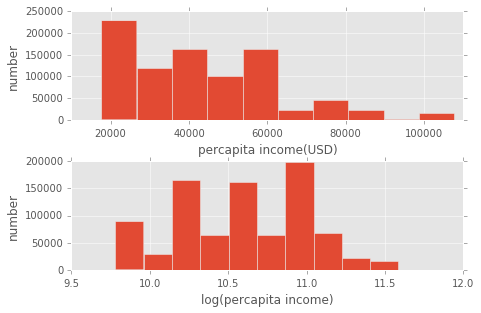
\includegraphics [width=0.48\textwidth]{pics/percapita_income_log.png}
\caption{}
\end{center}
\end{figure}

\section{Methods}
\subsection{Classification Algorithms}
Our choice of classification algorithm considers number of training samples, independence among features, linear separability as well as overfitting problem. Among various classifiers, Support Vector Machine(SVM) and K-Nearest Neighbors(KNN) are first abandoned because of their low computational efficiency. Our dataset has hundreds of thousands of entries and these algorithms would run for hours. Following are the algorithms selected for our classification experiments.\\

\subsubsection{Logistic Regression}
Logistic regression is a pretty well-bahaved classification algorithm that can be applied as long as predictors are roughly linear. We assume that our preprocessing have constructed a linear separable feature set and properly scaled numeric features. It is fast, and less vulnerable to overfitting by applying a simple 'l2' penalty function. 

Logistic regression employs a 'logit' model: $$ln\frac{p}{1-p}=\textbf{a} + \textbf{B}X + e$$ where p is probability that event $Y = \textbf{a} + \textbf{B}X + e$ happens. The fitting goal is to make likelihood $$L = Prob(p_1 * p_2 * ... p_n)$$ as large as possible by finding the coefficients $(\textbf{a}, \textbf{B})$. The log of $L$, namely log likelihood is usually calculated instead of $L$ itself, since $log()$ is monotonic. The python sklearn library implemented logistic regression, and we use its result as the baseline of other classification experiments.

\subsubsection{Random Forest}
Random Forest is a variation of CART(Classification and regression trees) models. CART models are popular for several advantages. They are easy to interpret, as we can derive series of rules by post-processing the tree. They can handle mixed discrete and continuous inputs, which is a characteristic of our spatio-temporal dataset. They are also able perform automatic variable selection, and are relatively robust to outliers \cite{2}. 

However, CART models have evident disadvantages. They do not predict very accurately due to the greedy nature of the true construction algorithm. Also trees are unstable (also referred to as having high variance), because slight changes at input data could be escalated significantly as the tree grow. One approach to reduce the variance of an estimator is aggregating together many estimates. We can train M different trees on different randomly chosen subset of the data, and then compute the ensemble $$f(x) = \sum_{m=1}^{M}{\frac{1}{M}f_m(x)}$$ where $f_m$ is the $m'$th tree. This technique is called bagging. While running the sample algorithm on subsets could result in highly correlated predictors, the base leaners can be de-correlated by randomly choosing subsets of training data. And this random-choosing regime is referred to as \textbf{random forest}. To improve its performance, Bayesian adaptive regression trees are often applied to performing Bayesian space ensembles.\\

\subsubsection{Gradient Boost Tree}
Boosting is a greedy algorithm for fitting adaptive basis-function models. Gradient Boosting derives a generic loss function: $$\hat{f}=\underset{f}{\mathrm{argmin}} L(f)$$ where $f=(f(x_1),...,f(x_N))$ are the weak learners. This is solved with gradient decent stage by stage. At step m, let $g_m$ be the gradient of $L(f)$ evaluated at $f=f_{m-1}$:
$$g_{im} = {[\frac{\Delta L(y_i, f(x_i))}{\Delta f(x_i)}]}_{f=f_{m-1}}$$ 
Then the update is made: $$\textbf{f}_m = \textbf{f}_{m-1} - {\rho}_m \textbf{g}_m$$ where ${\rho}_m$ is the step length. The algorithm can be fitted to a weak learner to approximate the negative gradient signal. Hence we update 
$${\gamma}_m = \underset{\gamma}{\mathrm{argmin}} \sum_{i=1}^N{(-g_{im} - \phi (\textbf{x}_i;\gamma))^2}$$ The overall algorithm can be applied to log-loss or other loss functions such as Huber loss, which is more robust to outliers. The gradient boost algorithm could also over fit as there are no penalty functions like in Logistic Regression. It takes efforts to tune it for satisfactory performance.\\

\subsection{Time Series}
A time series is a sequence of data points with continuous time interval and successive measurements made over a time interval. Time series analysis comprises approaches for extracting meaningful statistics and other characteristics of the data. And time series forecasting is using a model to predict future values based on previously recorded data. It has been applied to crime analysis for decades \cite{3}.

VAR models (vector autoregressive models) are desiged for multivariate time series. It view each variable as a linear combination of past lags of itself and past lags of other variables. The variables(number of crimes in our case) are collected in a 39*1 vector. At time $t$, define the vector as $y_t$, a  $p$-th order VAR, namely VAR(p), is $$y_t = c + A_1y_{t-1} + A_2y_{t-2} + ... A_py_{t-p} + e_t$$ where $y_{t-j}$ is called the $j-th$ lag of y, c is constant intercept and $e_t$ is an error term. The VAR model assumes the data is \textbf{weakly stationary} and above attributes of $e_t$ must hold
\begin{enumerate}
	\item $E(e_t) = 0$, zero mean error
	\item $E(e_t{e_t}') = \Omega$, the contemporaneous covariance matrix of $e_t$ is positive semidefinite.
	\item $E(e_t{e_{t-k}}') = 0$, for any positive k. There is no series correlation in error term.
\end{enumerate}
An Augmented Dickey-Fuller unit root test \cite{4} is often employ to test stationarity.  Using the library from statsmodel \cite{5} , we performed the ADF test on each category with constant, linear and quadratic trend.  We chose BIC(Bayesian Information Criterion) for penalty strictness. (results in Fig 4). There are 23 categories with scores below 5\% level, and we selected these categories for time series model construction.

\begin{figure}[H]
\begin{center}
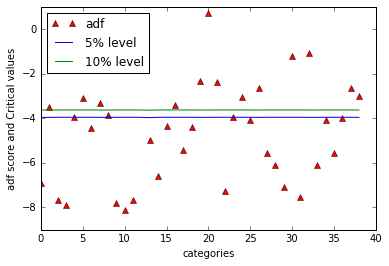
\includegraphics [width=0.48\textwidth]{pics/adf_test.png}
\caption{ADF test score against 5\% and 10\% threshold }
\end{center}
\end{figure}

\section{Experiments}
\subsection{Classification}
We have 878049 labeled spatio-temporal crime records, of which half are trained as training dataset, the rest are treated as test data to verify the accuracy of our classifiers. For each model, there are two kinds of prediction results. One is binomial labels(0 or 1) for each category, the other is possibility of each category. 
Following table displays the mean accuracy and log loss of each classification algorithms. For Random Forest and Gradient Boost Tree, we put the best results with highest accuracy and lowest log loss. 

We tried to incorporate demographic data to enrich our feature set, as introduced in the Datasets chapter. There are 18 demographic fields. To identify their influence, we constructed a matrix whose columns are demographic data and number of each category of crime, rows are neighborhood names. We computed its correlation matrix \textit{matcorr}. For each demographic field in \textit{matcorr}, we construct an array \textit{arrcorr} of its correlation with frequencies of all categories and compute the variance of \textit{arrcorr}. The larger variance it has, the stronger influence this demographic field has on crime category. Following table list eight most influential  entries. Apart from race, we see poverty percent, median home value and population density are also prominently informative.
\begin{table}[h]
\centering
\caption{Influential demographic data}
\label{my-label}
\begin{tabular}{|l|l|}
\hline
demographic feature                      & variance \\ \hline
latino ratio                             & 0.0282   \\ \hline
native\_hawaiian/pacific\_Islander ratio & 0.0250   \\ \hline
other/two\_or\_more\_races ratio         & 0.0243   \\ \hline
black ratio                                    & 0.0222   \\ \hline
poverty\_percent                         & 0.0168   \\ \hline
median\_home\_value                      & 0.0147   \\ \hline
population density                                  & 0.0143   \\ \hline
\end{tabular}
\end{table}

\begin{table}[h]
\centering
\caption{Accuracy and log loss of fitting result}
\label{my-label}
\begin{tabular}{|l|l|l|}
\hline
                    & accuracy & log loss \\ \hline
Logistic Regression & 0.3258        & 2.2176   \\ \hline
Random Forest       & 0.3376        & 2.2038   \\ \hline
Gradient BoostTree  & 0.3356        & 2.1866   \\ \hline
\end{tabular}
\end{table}

The table demonstrate that Random Forest yields the highest accuracy and Gradient BoostTree has lowest log loss. Their results did not vary much, even the plain logistic regression also reached an accuracy of 0.3258. There are in total 39 classes, the accuracy of 0.33 is actually not bad. We computed the predict-probability on the test dataset from Kaggle, which has 884263 crime unlabeled crime records. By the time of submission, we ranked 47th on the leaderboard \url{https://www.kaggle.com/c/sf-crime/leaderboard} among over 1200 submissions. 

\subsubsection{Tuning Random forest}
Our main efforts with Random Forest was to tun the hyper-parameters to mitigate overfitting. The most relevant parameter to this task was the maximum depth of the decision trees(weak classifiers)  of which the Random Forest is composed. Besides, the number of estimators could also affect fitting results.

Using Sklearn in Python, We first tried different number of estimators. Fig 5 plots accuracy and log loss as $scaled\_log\_loss = 0.3 + \frac{log\_loss}{100}$. As is shown in the picture, the mean accuracy increases and log-loss reduces as the estimator number increases from 10 to 60, but converges after that.
\begin{figure}[H]
\begin{center}
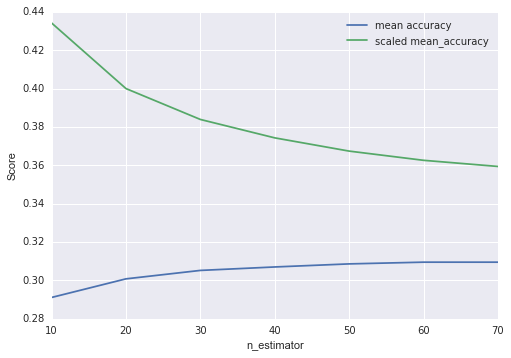
\includegraphics [width=0.48\textwidth]{pics/rf_p1.png}
\caption{Mean accuracy and scaled log loss}
\end{center}
\end{figure}

Considering time efficiency, we took 60 as the number of estimator for further training. To continue tuning the Random Forest algorithm and find its optimal max decision tree depth, we tried different max-depth with same number of estimator. Fig 6 shows the result. When max tree depth is 16, we gain the lowest log loss and highest accuracy.
\begin{figure}[H]
\begin{center}
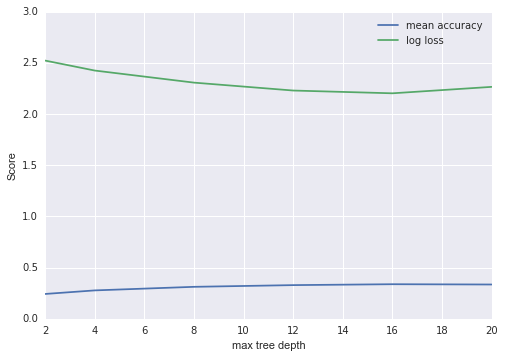
\includegraphics [width=0.48\textwidth]{pics/rf_p2.png}
\caption{Mean accuracy and scaled log loss}
\end{center}
\end{figure}

\subsubsection{Tuning GRBT}
The GRBT is supposed to have superior performance than Random Forest, but is painful to tune the parameters for optimal outcome. Generally, it is better to employ more decision trees for higher prediction accuracy and lower log loss. But our experiment results in fig 7 show that the best result occurs when the n\_estimator equals to 50, and increasing it does not improve the results.
\begin{figure}[H]
\begin{center}
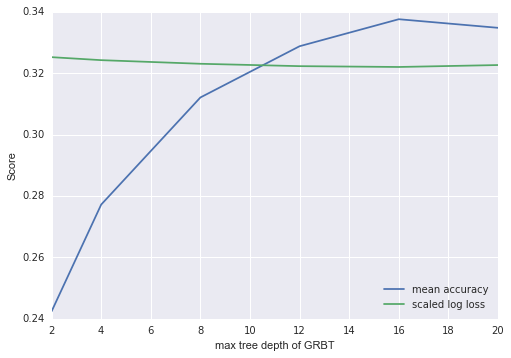
\includegraphics [width=0.48\textwidth]{pics/grbt_p1.png}
\caption{Mean accuracy and scaled log loss}
\end{center}
\end{figure}
We also compared the importance of different features with the 'gini importance' and selected the 20 most important predictors as shown in fig 8. \textbf{time}(hour of day) turn out to be the most important feature. The logodds account for the majority of influential features. Year also 
\begin{figure}[H]
\begin{center}
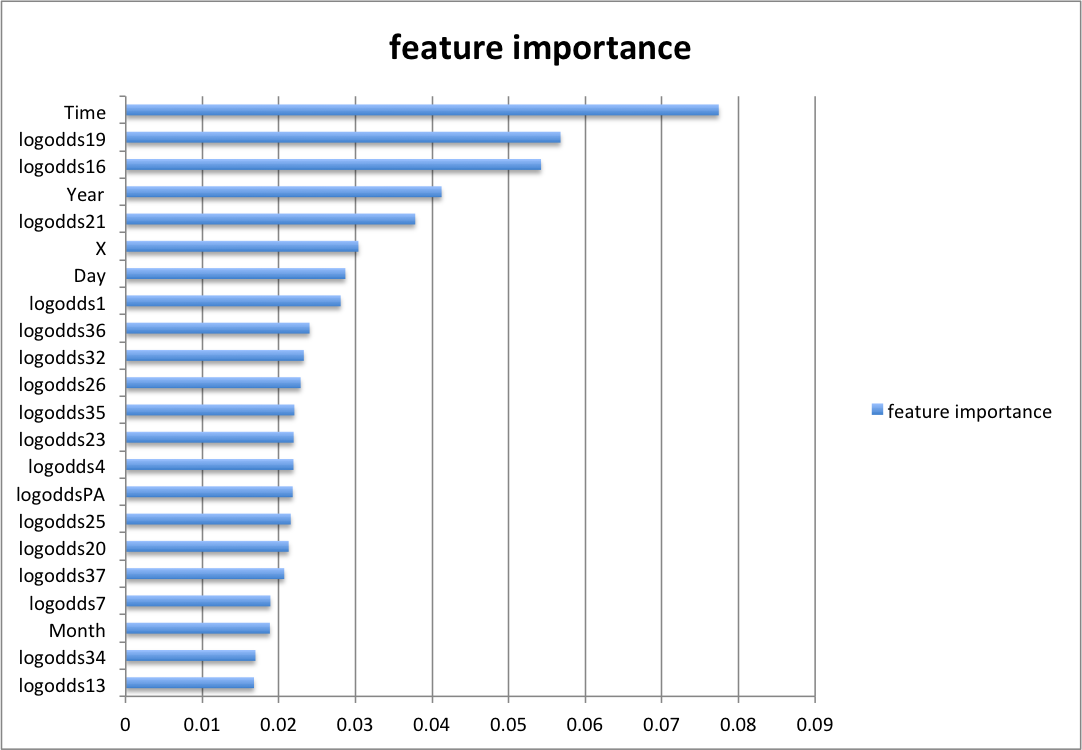
\includegraphics [width=0.48\textwidth]{pics/grbt_p2.png}
\caption{Mean accuracy and scaled log loss}
\end{center}
\end{figure}

\subsection{Time Series}
\subsubsection{Motivations}
Based on the stationarity test in previous chapter, the VAR{p} model is suitable for finding trends in the crime dataset. We selected 28 categories with low ADF score, and computed the pair-wise correlation among them. Fig 9 shows the heat-map of correlation matrix which computes the Pearson's r. In the heat-map, we can find large positively correlation coefficients, for example, BURGLARY \& ASSAULT, as well as negative coefficients like DRIVING UNDER THE INFLUENCE \& VEHICLE THEFT.
\begin{figure}[H]
\begin{center}
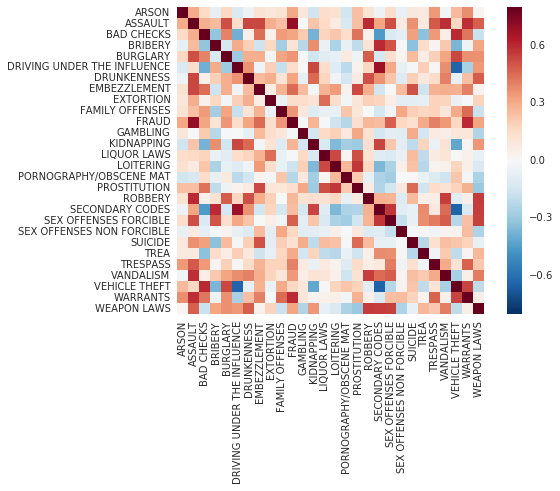
\includegraphics [width=0.48\textwidth]{pics/heat_map_time_series.png}
\caption{Heatmap of time series correlation matrix }
\end{center}
\end{figure}
Auto-correlation function(ACF) and Cross-correlation function(CCF) are also effective approaches to reveal statistical connections. Fig 10 demonstrate the CCF between category 'DRIVING UNDER THE INFLUENCE' and 'VEHICLE THEFT'. The increase of the first category precedes the decrease of the other. These kinds of correlations are further exploited in the correlation matrix.
\begin{figure}[H]
\begin{center}
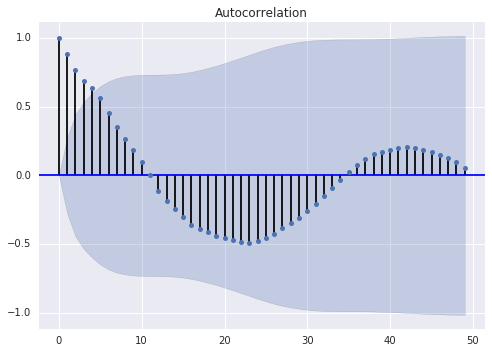
\includegraphics [width=0.48\textwidth]{pics/ccf_DRIVING_UNDER_THE_INFLUENCE_VEHICLE_THEFT.png}
\caption{CCF between 'DRIVING UNDER THE INFLUENCE' and 'VEHICLE THEFT'}
\end{center}
\end{figure}

\subsubsection{Model Selection}
Choosing the order $p$ for VAR(p) model is a feature selection problem. We tried different values of $p$ under two penalty criterions AIC(Akaike Information Criterion) and BIC. As is shown in Fig 11, with AIC, the penalty score is minimal when $p=2$. For BIC, the penalty is 30.88 at $p=1$ and 30.89 at $p=2$.
\begin{figure}[H]
\begin{center}
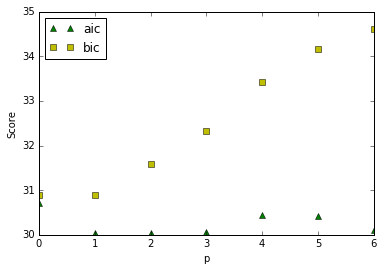
\includegraphics [width=0.48\textwidth]{pics/aic_bic.png}
\caption{aic/bic}
\end{center}
\end{figure}

\subsubsection{Fitting Model}
We choose $p=2$ and AIC penalty criterion for VAR(p) model fitting. And tried the model on "ASSAULT" time series. The first 40 time units were used for fitting, and the last 10 were forecasted. As Fig 12 shows, the model is not able to capture the exact quarterly variation, but it predicts the trend of increase or decrease in crime number correctly.
\begin{figure}%[H]
\begin{center}
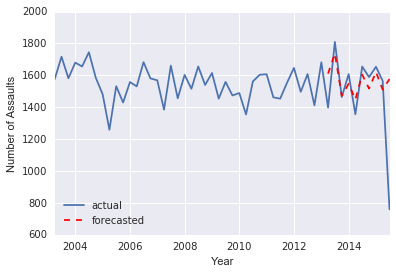
\includegraphics [width=0.48\textwidth]{pics/assault_forecast.png}
\caption{Forecast of 'ASSAULT'}
\end{center}
\end{figure}

\section{Related Work}
%TODO

\section{Conclusion}
In this paper, we worked on multi-class prediction and time series analysus on crime category in San Francisco. The dataset we employed included labeled spatio-temporal data from Kaggle and demographic data from US Census in 2010.

The prediction task achieved mean accuracy of around 33 percent, which ranked 47th among over 1200 submissions in Kaggle leaderboard. We compared Logistic regression, Random Forest and Gradient BoostTree algorithms. The ensemble tree methods are tuned with different max-tree-depth and number-of-estimators. The best fitting result was from Random Forest, while GRBT still possess the potential to excel other classifiers should it be further tuned with fine granularity. We involved demographic data to the classification task; however, it did not significantly improve the result.

We performed time series analysis on the spatio-temporal data with vector autoregression model. We found the optimal $p-lag$ with AIC and BIC penalty functions. From the heat-map, the crime category time series data also reveal correlation between different categories. The ADF test demonstrated that 23 out of 39 categories have more than 95\% probability to be stationary and we fitted VAR(p) model on these categories. The VAR(p) model is also able to predict trends of category number changes.

\section{Ackknowlegement}
I would like to deeply thank Professor D. Stott Parker for his advice on feature selection and preprocessing, which facilitated my preprocessing with demographic data.\\


\begin{thebibliography}{1}

\bibitem{1}
https://www.kaggle.com/c/sf-crime

\bibitem{2}
Murphy, Kevin P. Machine learning: a probabilistic perspective. MIT press, 2012.

\bibitem{3}
Greenberg, David F. "Time series analysis of crime rates." Journal of Quantitative Criminology 17.4 (2001): 291-327.

\bibitem{4}
Said, Said E., and David A. Dickey. "Testing for unit roots in autoregressive-moving average models of unknown order." Biometrika 71.3 (1984): 599-607.

\bibitem{5}
Seabold, Skipper, and Josef Perktold. "Statsmodels: Econometric and statistical modeling with python." Proceedings of the 9th Python in Science Conference. 2010.

\end{thebibliography}


\end{document}


